% Aigerim's Beauty Salon — тестовое задание Product Engineer
% Компилировать: pdfLaTeX (Overleaf по умолчанию).
% Скриншоты должны лежать рядом с именами: 00-landing.png ... 08-admin.png

\documentclass[11pt,a4paper]{article}

\usepackage[utf8]{inputenc}
\usepackage[T2A]{fontenc}
\usepackage[russian]{babel}
\usepackage[a4paper,margin=2cm]{geometry}
\usepackage{graphicx}
% картинки ищем и в корне (Overleaf), и в docs/screens (локально)
\graphicspath{{./}{docs/screens/}}
\usepackage{float}
\usepackage{booktabs}
\usepackage{tabularx}
\usepackage{enumitem}
\usepackage{xcolor}
\usepackage{textcomp}
\usepackage[hidelinks]{hyperref}

\definecolor{brand}{HTML}{C2306B}
\definecolor{ink}{HTML}{2A1F25}

\newcommand{\arr}{\textrightarrow{}}
\newcommand{\shot}[2]{%
  \begin{minipage}[t]{0.31\textwidth}\centering
    \includegraphics[width=\linewidth]{#1}\\[2pt]
    {\footnotesize #2}
  \end{minipage}}

\setlist{nosep,leftmargin=1.4em,topsep=2pt}
\setlength{\parindent}{0pt}
\setlength{\parskip}{5pt}

\title{\vspace{-1.5cm}\textbf{\color{brand}Aigerim's Beauty Salon — онлайн-запись}}
\author{Тестовое задание Product Engineer}
\date{}

\begin{document}
\maketitle
\vspace{-1cm}

\begin{center}
\begin{tabular}{ll}
\textbf{Кликабельный прототип:} & \href{https://slot-jet.vercel.app}{https://slot-jet.vercel.app} \\
\textbf{Код (фронт + бэк):} & \href{https://github.com/bazenovaalima-sketch/slot_reserve}{github.com/bazenovaalima-sketch/slot\_reserve} \\
\end{tabular}
\end{center}

\hrulefill

\section{Проблема и пользователь}

\textbf{Запрос Айгерим (как пришёл):} хаос с записью, двойные брони, мастера не в курсе, неявки, сгорающие слоты, гугл-календарь не зашёл, не хочет CRM «на сто кнопок».

\textbf{Настоящая боль (что под запросом):} Айгерим теряет \textbf{деньги} (пустые слоты от неявок и поздних отмен) и \textbf{нервы} (ручная синхронизация переписки \arr{} бумажного журнала \arr{} голов трёх мастеров). Корень один — \textbf{нет единого источника правды о расписании}. Запись живёт в WhatsApp, директе, журнале и в голове, поэтому накладки и потери неизбежны.

\textbf{Пользователи и роли:}
\begin{itemize}
  \item \textbf{Владелица/админ (Айгерим)} — главный пользователь и плательщик. Хочет перестать вести запись вручную и видеть деньги/загрузку.
  \item \textbf{Мастер ($\times$3)} — хочет в телефоне видеть «что у меня сегодня», без CRM-обвеса.
  \item \textbf{Клиентка} — хочет записаться за 30 секунд без переписки.
\end{itemize}

\textbf{JTBD:} «Когда клиентка хочет записаться — дай ей занять реально свободный слот за 30 секунд без переписки, так чтобы Айгерим не трогала журнал, мастер видел свой день, а освободившийся слот не сгорал».

\textbf{Приоритет болей (что берём первым и почему):}
\begin{enumerate}
  \item \textbf{Накладки + ручной ввод} — берём первой. Это корень: убери переписку как канал записи и сделай единый календарь с защитой от пересечений — исчезает и двойная бронь, и «мастер не знал». Самый дешёвый и острый wedge.
  \item \textbf{Неявки} — вторая. Депозит + напоминания.
  \item \textbf{Сгорающие слоты от отмен} — третья. Лист ожидания + автозаполнение.
\end{enumerate}

\textit{Пока запись идёт через переписку, любые напоминания и листы ожидания бессмысленны — нет источника правды. Сначала переносим запись в систему, потом наслаиваем борьбу с потерями.}

\section{Скоуп и решение}

\textbf{Идея:} одна \textbf{ссылка-запись} салона (в bio инстаграма / в ответ в WhatsApp). Клиентка выбирает услугу \arr{} мастера (или «любого») \arr{} видит только реально свободные слоты \arr{} вносит депозит \arr{} готово. Запись падает в \textbf{единый календарь}, который физически не даёт двойную бронь. Мастер видит свой день. Депозит и напоминания режут неявки. Отмена в один тап освобождает слот.

\textbf{v1 — что строим:} публичная страница записи; единый календарь с анти-накладкой; услуги и рабочие часы мастеров; депозит против неявок; WhatsApp-напоминание + подтверждение клиентом; кабинет студии (день по мастерам); отмена клиентом по ссылке.

\textbf{Что НЕ строим в v1 (смелость выкинуть):} полноценную CRM (карточки, история, теги, лояльность); аналитику и отчёты; зарплаты мастеров и склад; мультифилиалы и роли с правами; нативные приложения; прямую интеграцию с WhatsApp/Instagram API (v1 — просто ссылка).

\textbf{Допущения:} одна студия, $\leq$5 мастеров, услуги фиксированной длительности; слоты шагом 30 мин; один часовой пояс (Asia/Almaty); клиент идентифицируется телефоном, без регистрации; язык — русский.

\textbf{Компромиссы:} нет авторизации клиента \arr{} отмена/подтверждение по уникальной ссылке; оплата депозита и отправка напоминаний в прототипе \textbf{замоканы} (без реального Kaspi/WhatsApp-провайдера) — показана механика, в коде помечены точки интеграции.

\section{Требования и user flow}

\textbf{Функциональные:} публичная страница услуг/мастеров; расчёт свободных слотов (рабочие часы $-$ записи, под длительность услуги); создание записи с \textbf{атомарной} проверкой пересечения; депозит-гейт перед бронью; подтверждение записи + ссылка управления; кабинет с днём по мастерам; отмена \arr{} слот свободен; напоминание + статус подтверждения.

\textbf{Нефункциональные:} никогда не показывать слот, ведущий к накладке (источник правды — БД, проверка на сервере); мобайл-фёрст, без регистрации; понятные состояния (занято/выбрано/ошибка); идемпотентность создания.

\textbf{User flow по ролям:}
\begin{itemize}
  \item \textbf{Клиентка:} ссылка \arr{} услуга \arr{} мастер/«любой» \arr{} дата+время (только свободное) \arr{} имя+телефон \arr{} депозит \arr{} успех + превью напоминания.
  \item \textbf{Мастер:} своя ссылка \arr{} день списком \arr{} детали клиента \arr{} «пришёл / не пришёл».
  \item \textbf{Админ:} все записи всех мастеров, ручная отмена, действие «Напомнить», статусы депозита/подтверждения.
\end{itemize}

\textbf{Краевые случаи (покрыты):}
\begin{itemize}
  \item \textbf{Гонка за слот} — двое жмут «подтвердить» на один слот \arr{} выигрывает первый, второму честная ошибка «слот только что заняли».
  \item \textbf{Отмена} — слот освобождается (в v2 уходит первому из листа ожидания).
  \item \textbf{Неявка} — отметка no\_show; при оплаченном депозите помечается «депозит удержан».
  \item \textbf{Выходной/отпуск мастера} — его слоты исчезают из выдачи.
  \item \textbf{Запись в прошлое / впритык} — слоты раньше «сейчас» не показываются.
  \item \textbf{Услуга длиннее остатка смены} — не показываем слот, который не помещается до конца дня.
\end{itemize}

\section{Нарезка на релизы и модули}

\textbf{Модули:} A. Каталог; B. Расписание; C. Движок доступности; D. Бронирование (анти-накладка); E. Витрина клиента; F. Кабинет мастера/админа; G. Уведомления; H. Анти-потери (депозит, лист ожидания, no-show); I. Каналы (WhatsApp/Instagram, аналитика).

\renewcommand{\arraystretch}{1.3}
\begin{tabularx}{\textwidth}{@{}l X l@{}}
\toprule
\textbf{Релиз} & \textbf{Что входит} & \textbf{Модули} \\
\midrule
\textbf{v1 / Now} & Самозапись по ссылке, календарь без накладок, депозит, напоминание + подтверждение, кабинет, отмена & A--H (частично) \\
\textbf{v2 / Next} & Реальные WhatsApp/SMS-напоминания, лист ожидания + автозаполнение освободившихся слотов & G, H \\
\textbf{v3 / Later} & Интеграции с WhatsApp/Instagram, аналитика загрузки, постоянные клиенты, лояльность & I \\
\bottomrule
\end{tabularx}

\textbf{Почему именно это в v1:} без единого источника правды (C+D) ничего из остального не работает; депозит и напоминания (H, G) дают самый быстрый возврат денег и дёшевы поверх готового календаря.

\section{Прототип — флоу и почему}

\textbf{Ключевой флоу: самозапись клиентки} (услуга \arr{} мастер \arr{} время \arr{} депозит \arr{} успех). Почему он:
\begin{itemize}
  \item Это \textbf{wedge} — точка, где умирают сразу все боли (хаос переписки, двойные брони, «мастер не знал»).
  \item Это экран, которого касается клиент \arr{} на нём видно вкус и UX.
  \item Самодостаточен: кликабелен от начала до подтверждения.
\end{itemize}
Собран \textbf{фронт + бэк целиком} (не мокап): реальная БД, движок доступности и защита от двойной брони на сервере.

\textbf{Чем отличается от обычных «записей»:}
\begin{itemize}
  \item \textbf{Депозит против неявок} — бронь подтверждается мини-предоплатой ($\sim$30\%, зачитывается в стоимость). При неявке в кабинете видно «депозит удержан».
  \item \textbf{Умные напоминания} — на экране успеха клиент сразу видит превью WhatsApp-сообщения с кнопками «Подтверждаю / Перенести»; подтверждение загорается в кабинете.
\end{itemize}

\begin{figure}[H]
\centering
\shot{00-landing.png}{Лендинг салона}\hfill
\shot{01-service.png}{Выбор услуги}\hfill
\shot{02-master.png}{Выбор мастера}
\caption{Флоу самозаписи (1/3): вход \arr{} услуга \arr{} мастер.}
\end{figure}

\begin{figure}[H]
\centering
\shot{03-datetime.png}{Дата и время}\hfill
\shot{04-contacts.png}{Контакты}\hfill
\shot{05-deposit.png}{Депозит (мок-оплата)}
\caption{Флоу самозаписи (2/3): время \arr{} контакты \arr{} депозит.}
\end{figure}

\begin{figure}[H]
\centering
\shot{06-success.png}{Успех + напоминание}\hfill
\shot{07-manage.png}{Управление записью}\hfill
\begin{minipage}[t]{0.31\textwidth}\centering\strut\end{minipage}
\caption{Флоу самозаписи (3/3): подтверждение и управление записью.}
\end{figure}

\begin{figure}[H]
\centering
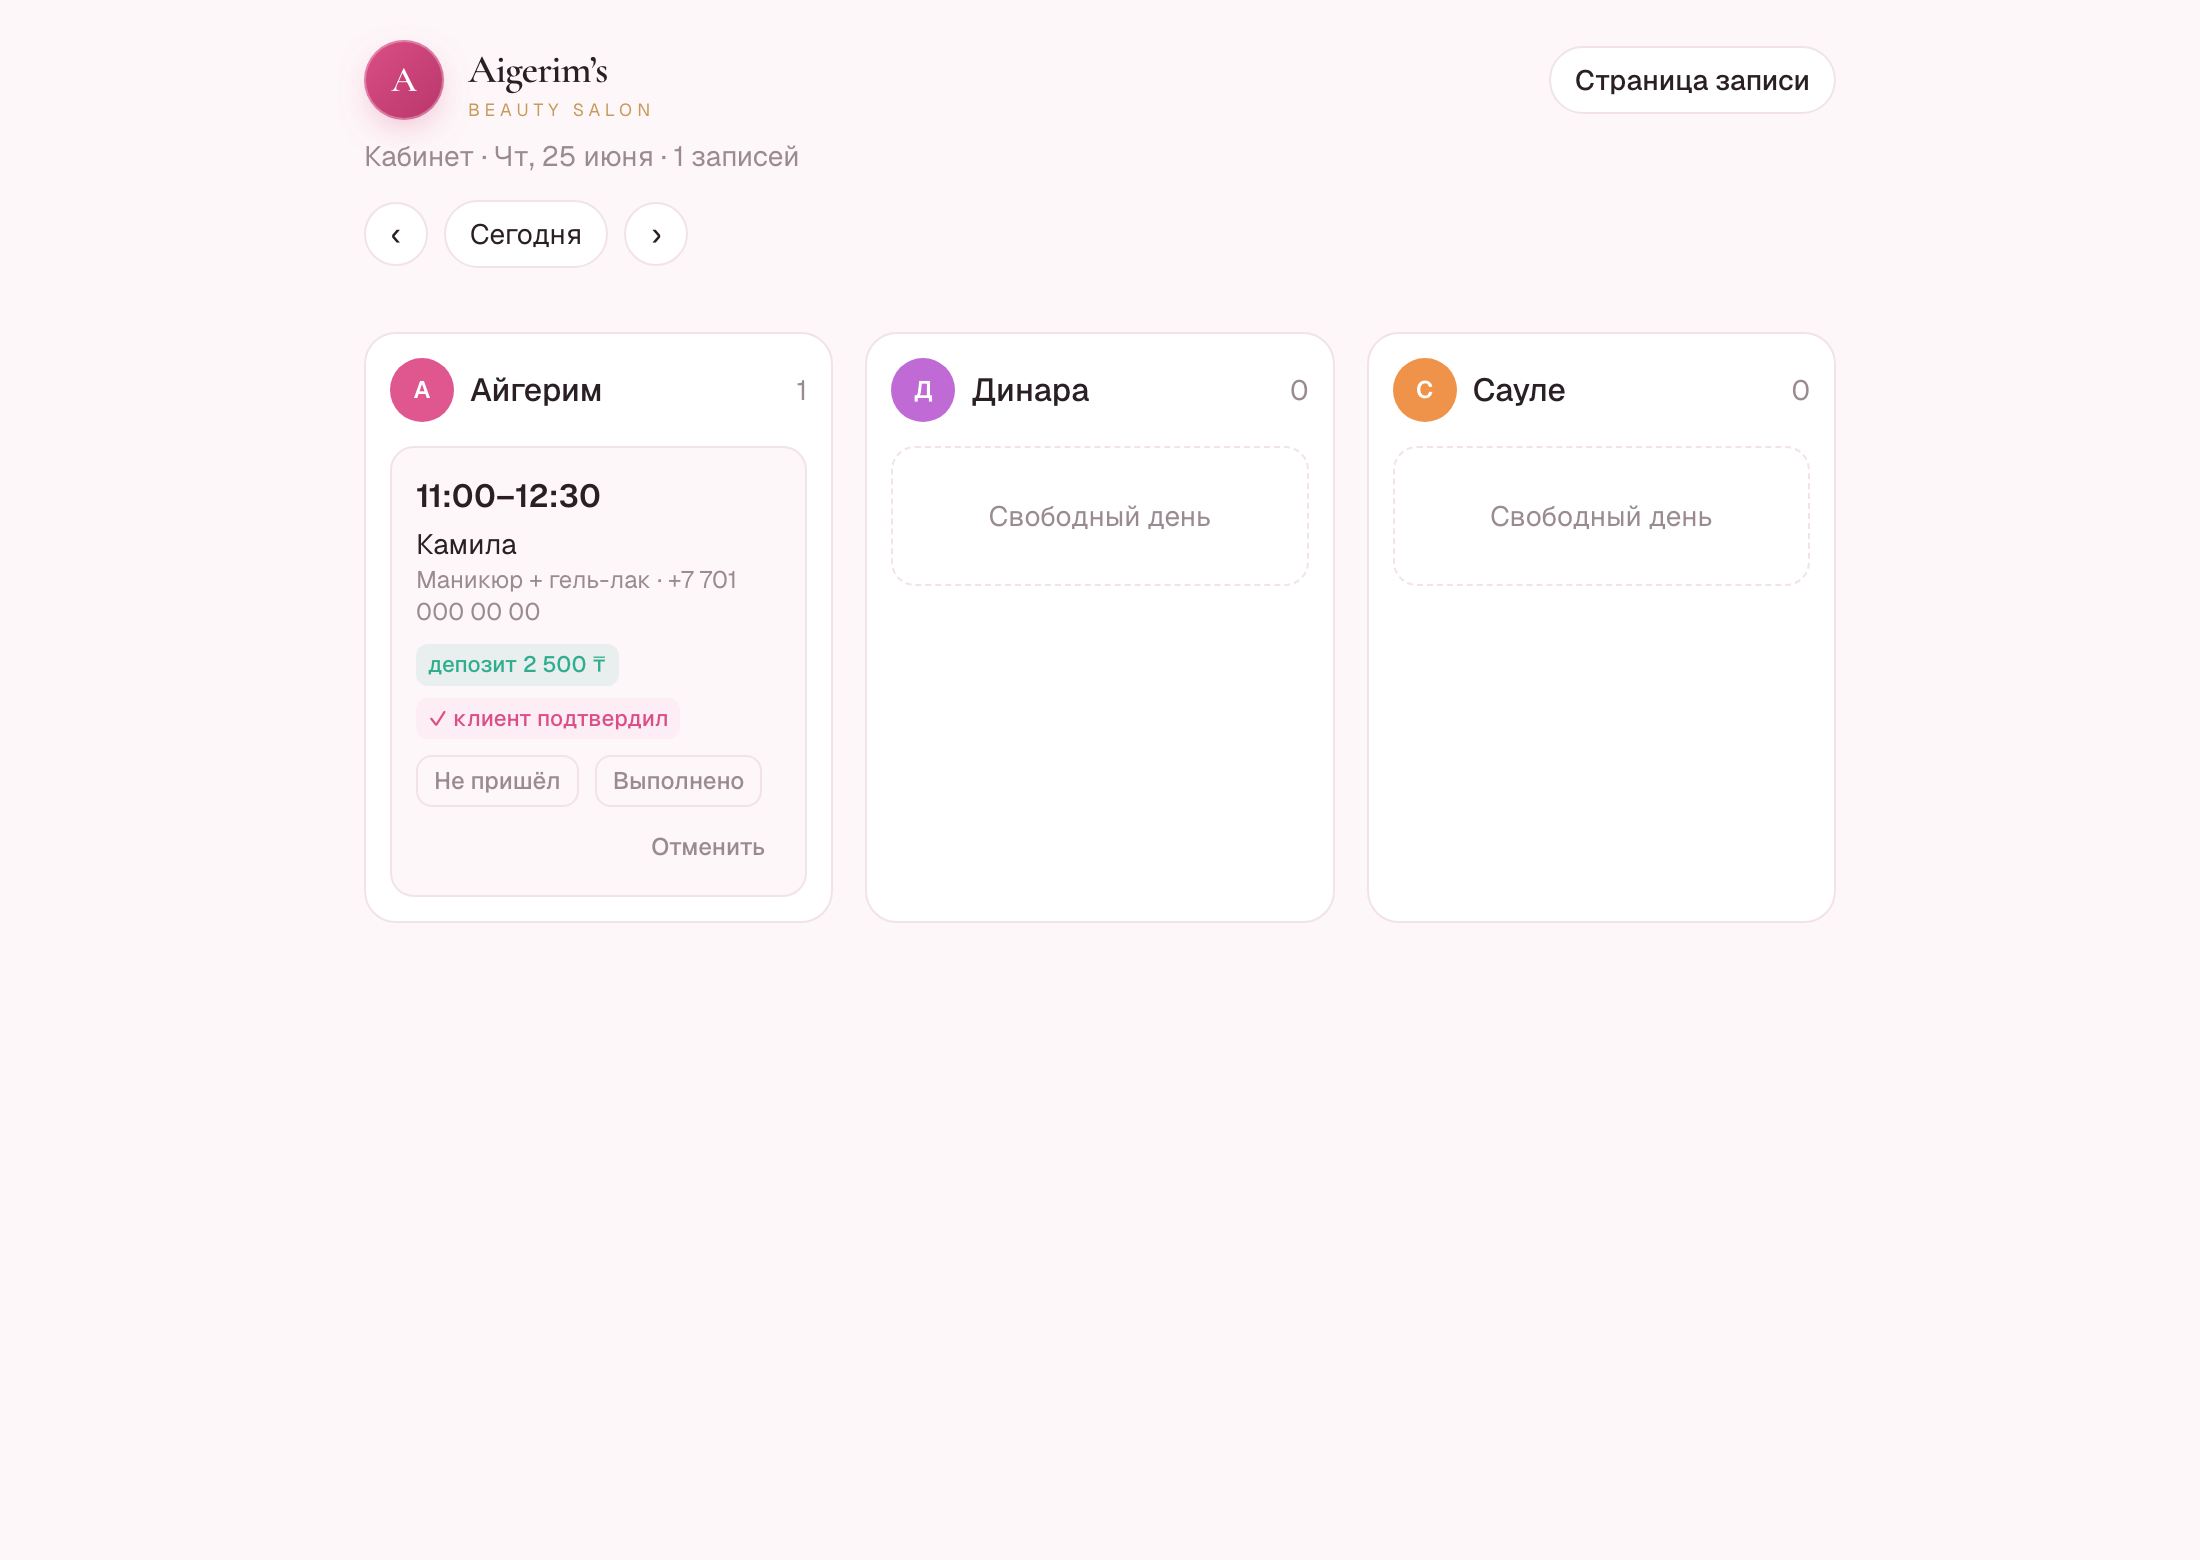
\includegraphics[width=0.92\textwidth]{08-admin.png}
\caption{Кабинет студии: день по мастерам, бейджи депозита и подтверждения, действия.}
\end{figure}

\section{Стек и архитектура}

Next.js 16 (App Router, Server Actions); React 19; Prisma 7; PostgreSQL (Neon); Tailwind v4; деплой Vercel. Фронт и бэк в одном репозитории; доступность и анти-накладка считаются на сервере (источник правды — БД), проверка пересечения — внутри транзакции.

\section*{Рефлексия}

\textbf{На что ушло время:} $\sim$60\% — продуктовое мышление (найти настоящую боль, выбрать острый wedge, честно выкинуть лишнее) и $\sim$40\% — один доведённый флоу с реальным фронтом и бэком: движок доступности, защита от двойной брони в транзакции, депозит и напоминания.

\textbf{Что сделал бы за ещё 3 дня (по приоритету):} (1)~\textbf{Лист ожидания + автозаполнение} освободившихся слотов — прямой возврат денег и главная боль клиента, которую конкуренты не закрывают; (2)~\textbf{реальные} WhatsApp-напоминания и Kaspi-оплата депозита через провайдеров; (3)~редактирование рабочих часов, выходных и услуг из кабинета, а не из сида.

\end{document}
